\section{Problem 1}
\label{part1}
\subsection*{Question}
\begingroup
\begin{verbatim}
Create a blog-term matrix.  Start by grabbing 100 blogs; include:

http://f-measure.blogspot.com/
http://ws-dl.blogspot.com/

and grab 98 more as per the method shown in class.

Use the blog title as the identifier for each blog (and row of the
matrix).  Use the terms from every item/title (RSS) or entry/title
(Atom) for the columns of the matrix.  The values are the frequency
of occurrence.  Essentially you are replicating the format of the
"blogdata.txt" file included with the PCI book code.  Limit the
number of terms to the most "popular" (i.e., frequent) 500 terms,
this is *after* the criteria on p. 32 (slide 7) has been satisfied.

Create a histogram of how many pages each blog has (e.g., 30
blogs with just one page, 27 with two pages, 29 with 3 pages and 
so on).
\end{verbatim}
\subsection{Answer}
\begin{enumerate}
\item The script shown in Listing \ref{lst:blogsScript} outputs a list of 100 random blogs in to a file . 
\item The script show in Listing \ref{lst:atomFeedsScript} outputs a list of atom feed for the respective blog. The atom feed grabbed will give only 25 entries by default.
\item After little research I found out that we can set the max limit by adding \emph{max-result=1000}. So I appended the maximum limit to each atom feed extracted from Listing \ref{lst:atomFeedsScript}. 
\item The scripts were written based on the technique that is taught in the class.
\item To get the words from each feed I used \emph{Segaran's generatefeedvector.py} from Program Collective Intelligence Text book. 
\item I modified the \emph{generatefeedvector.py} code to get the popular 500 words from all the atom feed.
\item I included a piece of code at line 34 in Listing \ref{lst:code-500words}to eliminate the words which falls under the stop words, the stop word list used is the ``MySql full-text stopwords''. 
\item The code does not handle the entries if the entries for the blog is beyond 500 as the maximum limit of the entries for an atom feed is limited to only 500 entries at a time. 
\item So to get the entries which are beyond 500, I wrote a piece of code from line 37 to 48 which handles that scenario. I am considering the 2000 entries for an atom feed and extracting the words from all those entries.  
\item To get the most popular words among all the blogs, firstly I am keeping track of the occurrence of each word in all the blogs.
\item So that I can pick only the top 500 words by sorting the words based on the occurrence value. 
\item This is implemented at lines 106 -108 and  121-124 in Listing \ref{lst:code-500words}. And then I am limiting down the word to top 500 words only.
\item The script shown in Listing \ref{lst:code-500words} outputs the matrix in expected format which is stored in \emph{blogdata-500.txt} which is used for each subsequent question in this assignment, this file is uploaded in the github. 
\item To get the number of pages in each blog, I wrote a small python code as shown in Listing \ref{lst:blogVsPages} which outputs the file \emph{PagesInBlogs.txt}
\item The R script shown in the Listing \ref{lst:r-script} generates a Histogram shown in Figure \ref{Histogram 1} for Blogs Vs no of Pages. 
\item From the Histogram in Figure \ref{Histogram 1}, it's pretty clear that 30 blogs out of 100 have pages between 100 and 200, and only couple of blogs have pages between 2800 and 3000. 
\end{enumerate}

\lstinputlisting[language=bash, frame=single,breaklines=true, caption={Shell Program for getting 100 blogs}, label=lst:blogsScript, captionpos=b, numbers=left, showspaces=false, showstringspaces=false, basicstyle=\footnotesize]{questions/q1/getblogs.sh}

\lstinputlisting[language=bash, frame=single,breaklines=true, caption={Shell Program for getting atom feed for the blogs}, label=lst:atomFeedsScript, captionpos=b, numbers=left, showspaces=false, showstringspaces=false, basicstyle=\footnotesize]{questions/q1/getRss.sh}

\newpage

\lstinputlisting[language=python, frame=single,breaklines=true, caption={Python code for grabbing popular 500 words from 100 atom feeds},captionpos=b, numbers=left, showspaces=false,label=lst:code-500words, showstringspaces=false, basicstyle=\footnotesize]{questions/q1/top500Words-2000pages.py}

\lstinputlisting[language=python, frame=single,breaklines=true, caption={Python code for grabbing number of pages for each blog},captionpos=b, numbers=left, showspaces=false,label=lst:blogVsPages, showstringspaces=false, basicstyle=\footnotesize]{questions/q1/noOfPages.py}
\newpage
\lstinputlisting[language=R, frame=single,breaklines=true, caption={R Script for generating a Histogram},captionpos=b, numbers=left, showspaces=false,label=lst:r-script, showstringspaces=false, basicstyle=\footnotesize]{questions/q1/R/historgram.R}

\begin{figure}[ht]    
    \begin{center}
        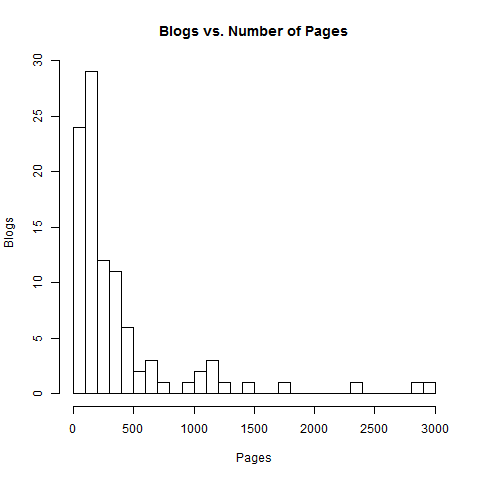
\includegraphics[scale=0.60]{questions/q1/R/q1-histogram1.png}
        \caption{Histogram showing Blogs Vs No of Pages}
        \label{Histogram 1}
    \end{center}
\end{figure}

\newpage